
%----------------------------------------------------------------
%
%  File    :  open_source.tex
%
%  Authors :  ???
% 
%  Created :  7 Sept 2019
% 
%  Changed :  7 Sept 2019
% 
%---------------------------------------------------------------

\section{Open Source Lösung}
\label{sec:open_source}

Im Gegenzug zu teurer Spezial-Hardware und nicht frei zugänglicher Software, gibt es auch sogenannte Open-Source Lösungen. Grundsätzlich kann eine Software als Open-Source bezeichnet werden, wenn der Quellcode dieser veröffentlicht wird. Im Gegenzug, zur einfachen Bereitstellung einer rein ausführbaren Datei.
Des Weiteren wird frei zugängliche Software oftmals mit eingeschränkten, oder keinen Beschränkungen weitergegeben. Diese ist daher oftmals frei und kostenlos zu verwenden und somit auch erweiter- und veränderbar. \cite{gacek2004many}

\subsection{OpenAirInterface - OAI}
Im konkreten Anwendungsfall, ermöglicht es eine solche Software, kostengünstig ein eigenes LTE-Netzwerk aufzubauen. 
Ganz ohne Hardware geht dies natürlich nicht, jedoch würde ein Modul für etwa 1500,- ausreichen um ein entsprechendes Netz aufzubauen. Ein solches Software Defined Radio (SDN) wäre etwa das "Flexible, next-generation, open source software-defined radio"\ von LimeMicrosystems, welches im Zuge einer Crowdfunding-Aktion realisiert wurde \cite{CroudLime01}. 

Mit einem SDN werden Anteile der Signalverarbeitung mittels Software realisiert. Dies kann von dedizierter Hardware unterstützt werden. Des weiteren bietet es eine gewisse Flexibilität zu einer reiner Hardware Lösung, da Software veränderbar ist \cite{jondral2005software}. 

Das OpenAirInterface ist ein Projekt der OpenAirInterfaceTM Software Alliance (OSA), welches eine Open Source Lösung zur Verfügung stellt \cite{OpenAir19}.

Dabei wird die Lösung in zwei Projekte unterteilt. 
\begin{itemize}
	\item eNodeB (eNB): “openairinterface5G”
	\item evolved packet core (EPC): “openair-cn”
\end{itemize}

OpenAirInterface ist die erste Open-Source Software Platform welche eines LTE Systems welches den vollen Protokollstack des 3GPP Standards, inklusive E-UTRAN und EPC unterstützt.
Dabei kann dies sowohl für das Erstellen eines eigenen LTE Netzes, als auch das Überwachen (Monitoring) verwendet werden \cite{nikaein2014openairinterface}.
Des Weiteren ist es möglich, Performance-Analysen durchzuführen und dabei Einblicke zu erhalten, wie sich ein rasch skalierendes System verhält. 

\begin{figure*}[ht]
	\centering
	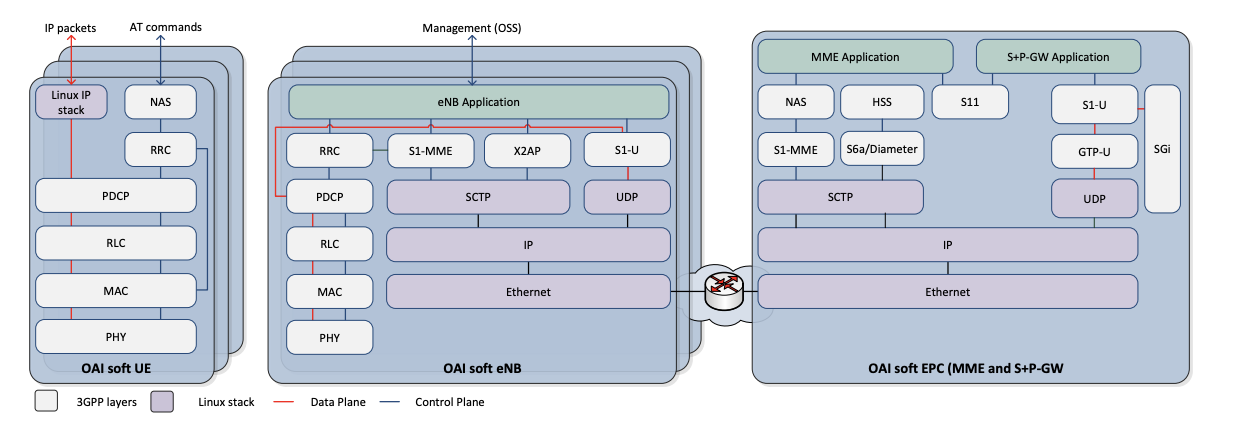
\includegraphics[width=0.7\linewidth]{BestandTeileOAI}
	\caption{Übersicht LTE Module in den jeweiligen Projekten \protect\cite{openAirInterfaceOverview19}}
	\label{fig:modulesOAI}
\end{figure*}


Abbildung \ref{fig:modulesOAI} zeigt die schematische Implementierung des LTE Protokoll Stacks in OAI.
Dem Hersteller zufolge wurden hiermit auch diverse Tests durchgeführt. So wurde Beispielsweise OAI eNB mit kommerziellen Huawei Geräten getestet, bei welchen LTE aktiviert wurde (E392, E398u-1) und OAI-UE mit CMW500 (Ericsson on com4Innov network).

Die OpenAirInterface Open Source Initiative bietet sowohl Unterstützung für eNodeB (eNB), User Equipment (UE) wie auch Evolved Packet Core (EPC) an. Zudem wird, neben dem oben erwähnten Lime SDR auch noch ETTUS  USRP und ExpressMIMO2 unterstützt. Des Weiteren erlaubt OAI hierbei auch die Unterstützung kommerzieller Ausrüstung \cite{kaltenberger2019openairinterface}. Somit ist man hier nicht auf ein spezielles SDR eingeschränkt.

\subsection{srsLTE}
srsLte bietet eine sehr modulare Architektur, um auch rasch neue Standards einfließen lassen zu können. Diese ist in funktionale Module aufgebaut. Damit wird hier auch bereits ein Satz an Beispielanwendungen geboten, welche für eigene Anwendungen angepasst werden können \cite{puschmann2017implementing}. 
Des Weiteren sind auch Anpassungen möglich, um zusätzliche Hardware zu unterstützen. 
Abbildung \ref{fig:modulessrsLTE} zeigt diesen modularen Aufbau.

\begin{figure*}[ht]
	\centering
	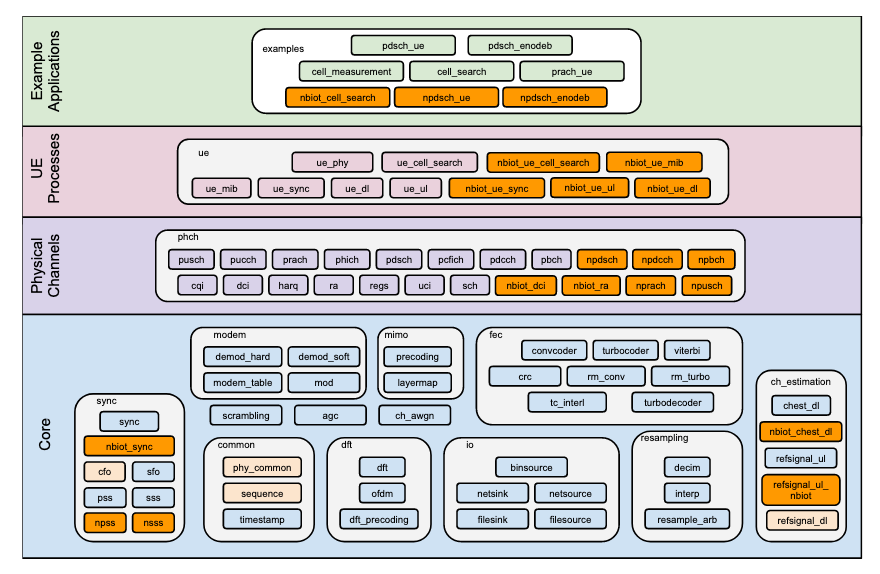
\includegraphics[width=0.7\linewidth]{ssrLTE_Module}
	\caption{Übersicht Architektur srsLTE \protect\cite{puschmann2017implementing}}
	\label{fig:modulessrsLTE}
\end{figure*}

Die Beispielanwendungen geben einen Überblick zum Betrieb als eNodeB (srsENB, srsEPC) sowie Informationen um dies als UE (srsUE) einsetzen zu können. Entwickelt wurde diese von Software Radio Systems, welche dieses Projekt auf Github zur Verfügung stellt \cite{githubSrSLTE}.

Die hohe Flexibilität und Anpassbarkeit ist auch Grund für Abwandlungen und andere Projekte, welches dies srsLTE als Basis verwenden. So ist etwa \nameref{tinyLTE} eines dieser genannten Projekte. Zudem wird die Software regelmäßig gewartet, was auch an den Codeänderungen im Repository zu erkennen ist. 

\subsection{tinyLTE}
\label{tinyLTE}
Eine weitere Open-Source Lösung ist tinyLTE. Auch dieses verwendet SDR, um größtmögliche Flexibilität und Offenheit zu bieten. Dabei unterstützt dies sowohl als LTE Client (UE) als auch Infrastruktur (eNB + EPC) \cite{eckermann2018tinylte}.

Der Vorteil dabei ist, dass hiermit ein gleichzeitiger Betrieb von beiden Anwendungsfällen möglich ist. In Kombination mit Hardware, welches 2 SDRs unterstützt, kann so ein einzelnes Gerät die volle Funktionalität anbieten. 
Beides basiert, mit geringen Änderungen, auf srsLTE \cite{gomez2016srslte}. 

Die Lösung von Philipp Gorczak sowie Fabian Eckermann wurde auf Github zur Verfügung gestellt. Eine Evaluierung im Betrieb wurde ebenfalls bereits getestet. Dabei ging es um die Kommunikation über LTE zwischen Fahrzeugen. 

\subsection{Unterschiede}
Alle drei erwähnten Lösungen bieten einen breiten Funktionsumfang und Unterstützung an. Unterschiede sind etwa in der getesteten Hardware zu erkennen. Sollte bereits bestehendes Equipment vorhanden sein, könnte dies ein Indikator für eine Präferenz darstellen. 
tinyLTE wurde speziell für die Kommunikation zwischen Fahrzeugen entwickelt und getestet. 